\section{Теоретические сведения}
В этой главе рассмотрены теоретические сведения человеческой речи, речевых признаках и общая схема алгоритма распознавания звука.

\subsection{Речь как объект распознавания}
Человеческая речь - результат выдыхания человеком из себя воздуха через рот или нос. При этом воздух, проходя по трахее и бронхам, вибрирует. Саму вибрацию человек может контролировать при помощи положения языка, усиления или ослабления выдыхаемого воздушного потока и степенью натяжения различных мышц. Таким образом, речевом аппарате человека две основные составляющие - генератор тонового сигнала и совокупность фильтров.

В конечном итоге речь представляет из себя колебания воздуха - звуковые волны определенной амплитуды. Волны улавливаются мембранами в приемниках звука. В случае человеческого уха происходит следующее. Звуковые волны проходят через наружное ухо в среднее и вызывают вибрацию барабанной перепонки. Колебания с барабанной перепонки передаются на маленькие слуховые косточки в среднем ухе. А со слуховых косточек — во внутреннее ухо. Когда эти колебания достигают улитки, они воздействуют на специальные клетки — волосковые. Волосковые клетки преобразуют колебания в электрические нервные импульсы. Слуховой нерв соединяет улитку с центрами слуха в головном мозге. Когда электрические нервные импульсы достигают головного мозга, они воспринимаются как звук и обрабатываются.

В случае с компьютером и подключенным к нему микрофоном - принцип схожий. Звуковые волны колеблют мембрану в микрофоне. Разница в положении мембраны замеряется в виде электрического сигнала при помощи, например, конденсатора.  Далее электрический сигнал, поступает по проводу в компьютер, и там проходит обработку.

Человеческая речь - довольно специфический звуковой сигнал. Человеческий голос в среднем имеет диапазон частот от 100Гц до 4000Гц. Чем выше частота звука, тем менее чувствительно к нему ухо человека. Еще одной особенностью является то, что для повышения громкости звука в 2 раза необходимо в 8 раз больше энергии.

Речь можно представить в виде последовательности предложений, а их в свою очередь в виде последовательности слов. Слова же состоят из фонем. В общем случае речь непрерывна, т.е. слова не отделяются друг от друга паузами, за исключением того требующих пунктационных особенностей. В этой работе не рассматривается общий случай. Здесь рассмотрен частный случай, когда речь состоит из отдельных слов, отделяемых друг от друга тишиной в понимании человеческой речи. Этот выбор был обусловлен командным типом системы распознавания, которая работает с отдельными словами.

\subsection{Речь в компьютерном представлении}
Каждая речевая команда с точки зрения звуковой записи в компьютере - это набор амплитудных значений, полученных с микрофона и записанных в звуковой файл.

\subsection{Общая схема алгоритма распознавания}
На рисунке \ref{fig:algo_scheme} представлена общая схема работы алгоритма распознавания речевых команд. Алгоритм разделен на два основных блока, обозначенных на рисунке как Блок 1 и Блок 2. На вход алгоритму поступает наборы амплитудных значений и соответствующие частоты дискретизации в формате wav. На выходе алгоритма - текстовое представление команды.

\begin{itemize}[leftmargin=2cm]
\item Блок 1 - блок, отвечающий за первоначальную обработку данных и приведение их к единому формату. 
\item Блок 2 - блок, отвечающий за классификацию унифицированных данных. Этот блок может работать в двух режимах: обучения и непосредственной работы. В режиме обучения меняются параметры алгоритма, которые влияют на конечный результат. В режиме непосредственной работы этого не происходит.
\end{itemize}


\begin{figure}[H]
  \[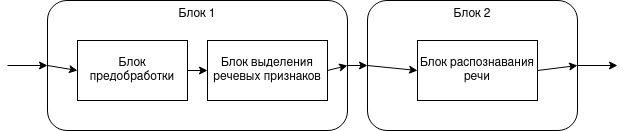
\includegraphics[scale=0.6]{algo_scheme.png}\]
  \caption{Общая схема работы алгоритма распознавания речевых команд}
  \label{fig:algo_scheme}
\end{figure}
